\chapter{Métodos}\label{chapter:Methods}


El canto de \emph{E.\,eileenae} ocurre durante la noche, 
cuando los machos se agrupan para vocalizar, con picos de 
actividad en los meses cálidos y lluviosos del año, y en las
horas de la tardenoche y la madrugada. Los datos empleados en 
esta investigación fueron obtenidos por un grupo de 
investigación liderado por el Dr. Roberto Alonso, de la 
Facultad de Biología de la Universidad de La Habana, mediante 
un conjunto de grabaciones de campo realizadas en la Reserva 
de la Biosfera “Sierra del Rosario”. Luego de identificar 
ciertos individuos de Colín y los sitios en los que 
habitualmente se ubicaban para emitir sus cantos, se 
colocaron nueve micrófonos (cada uno a aproximadamente un 
metro de su individuo más cercano) cuya activación remota 
permitió registrar la información acústica del coro. Todos los 
dispositivos, del mismo modelo y omnidireccionales, 
fueron activados simultáneamente para grabar durante 58 minutos 
consecutivos, seguidos por un intervalo de 2 minutos destinado a 
la descarga y almacenamiento de los datos adquiridos. Este 
ciclo se repitió cada hora, desde las 18:00 hasta las 06:00 
del día siguiente, durante tres noches consecutivas, entre el 
20 y el 23 de octubre de 2023. Como resultado, se conformó un 
\textit{dataset} estructurado en el que, por cada hora de 
grabación, se dispone de los nueve archivos correspondientes a 
los nueve micrófonos utilizados. Tal como se indicó 
previamente, los dispositivos fueron ubicados dentro de un 
área de aproximadamente 20 metros de radio.



Debido a que los micrófonos eran omnidireccionales y estaban situados 
relativamente cercanos entre sí, en cada uno se registraron no solamente
los cantos del individuo de Colín más próximo, sino también cantos de especímenes
cercanos, sonidos del ambiente natural de la zona, e incluso ruidos de 
agentes artificales como autos pasando por una carretera aledaña.
Esto planteó una serie de dificultades para el análisis de los datos,
como la de eliminar la información ruidosa, y la de distinguir y extraer
en cada audio los cantos del Colín que corresponden al micrófono en cuestión. 

De esta forma, se impuso emplear un método automático para “limpiar” los audios.
Además, para poder obtener las secuencias de cantos y estudiar los coros,
surgió la necesidad de diseñar procesos para discriminar correctamente
estos datos, y obtener una asigación Micrófono-Colín.   
También se debía verificar la correcta sincronización de las grabaciones,
pues a pesar de la activación remota y simultánea, posibles errores de medición
podrían comprometer la precisión de los resultados. En este capítulo
se describen los métodos utilizados para resolver tanto estos problemas
como el de modelar las interacciones del sistema. 

Con el objetivo de simplificar las explicaciones, se decidió 
asignar una letra entre la “a” y la “i” a cada uno de los micrófonos,
de modo que la correspondencia entre la notación original y la nueva 
queda de la siguiente forma:
\begin{itemize}
    \item Micrófono 10: a
    \item Micrófono 12: b\footnote{En los datos originales no existe micrófono 11.}
    \item Micrófono 13: c
    \item Micrófono 14: d
    \item Micrófono 15: e
    \item Micrófono 16: f
    \item Micrófono 17: g
    \item Micrófono 18: h
    \item Micrófono 19: i
\end{itemize}

Por lo tanto, una grabación en específico, por ejemplo la del 21 de octubre de 2023 a las 
19:00 horas, registrada por el micrófono “h”, será referida como “\texttt{20231021\_190000h}”.

Para la grabación se emplearon dispositivos AudioMoth, 
desarrollados como placas de circuito impreso de 58x48x18mm 
(80g con baterías), basados en un microcontrolador ARM 
Cortex-M4F con unidad de punto flotante y un micrófono MEMS 
bottom-ported. Cada unidad muestreó audio sin compresión WAV a 
velocidades de hasta 384kHz, almacenando los datos en tarjetas 
microSD de hasta 32GB. Gracias a su excepcional eficiencia 
energética (con consumos de 10-25mW durante la adquisición y 
80µW en reposo), 
resultaron idóneos para despliegues prolongados alimentados por 
tres pilas AA, manteniendo la sincronización y calidad 
requeridas para el estudio de los coros de \emph{E.eileenae} \cite{hill2018audiomoth}.


% region mel spectrograms
\section{Representación de audios con Mel-espectrogramas}
\label{sec:mel_spectrogramas}

La escala de mel es una escala perceptual de tono que aproxima la 
respuesta no lineal del oído humano a diferentes frecuencias. A 
diferencia de la escala lineal en Hertz (Hz), enfatiza la 
discriminación de frecuencias bajas (e.g., 100-1000 Hz) y 
comprime las altas (e.g., >4000 Hz), reflejando cómo los humanos 
perciben diferencias de altura tonal. Ampliamente utilizada en 
procesamiento de audio, permite representar señales acústicas 
en formatos espectralmente significativos llamados Mel-espectrogramas, 
facilitando la detección de patrones relevantes. \cite{zhang2021acoustic}
Un Mel-espectrograma se obtiene aplicando una ventana 
deslizante al audio, calculando la FFT en cada segmento, mapeando las bandas de 
frecuencia a la escala mel y, finalmente, tomando el logaritmo 
de la energía resultante \cite{zhang2021acoustic}. 

Para el análisis de las grabaciones se transformó cada archivo 
de audio en su correspondiente Mel-espectrograma,
buscando enfatizar las variaciones espectrales relevantes 
para el canto de \emph{E.\,eileenae} y facilitar la detección de 
los pulsos “CO” y “LIN” en los audios.

Para la generación de los Mel-espectrogramas se emplearon los 
siguientes parámetros, optimizados para cubrir el rango de 
frecuencias de los cantos de Colín (aprox. 1.8-3.1 kHz) \cite{alonso2001llamadas} 
y garantizar resolución temporal suficiente para distinguir 
emisiones consecutivas:
\begin{itemize}
  \item \texttt{hop\_length} = 512 (desplazamiento de ventana)  
  \item \texttt{n\_fft} = 6096 (número de puntos para calcular la FFT)  
  \item \texttt{n\_mels} = 128 (número de bandas mel a utilizar)  
  \item \texttt{f\_min} = 1600 Hz (frecuencia mínima mapeada)  
  \item \texttt{f\_max} = 4096 Hz (frecuencia máxima mapeada)  
  \item \texttt{sample\_rate} = 96000 Hz (tasa de muestreo de las grabaciones)  
\end{itemize}

En la Figura \ref{fig:mel_example} se muestra un 
Mel-espectrograma de un fragmento del audio 
\texttt{20231021\_190000h}. En él pueden identificarse 
claramente los instantes de emisión de la nota baja “CO” 
(fragmento en torno a la 20 banda de mel) y de la nota alta “LIN” 
(bandas intensas por encima de la 60).

\begin{figure}[ht]
  \centering
  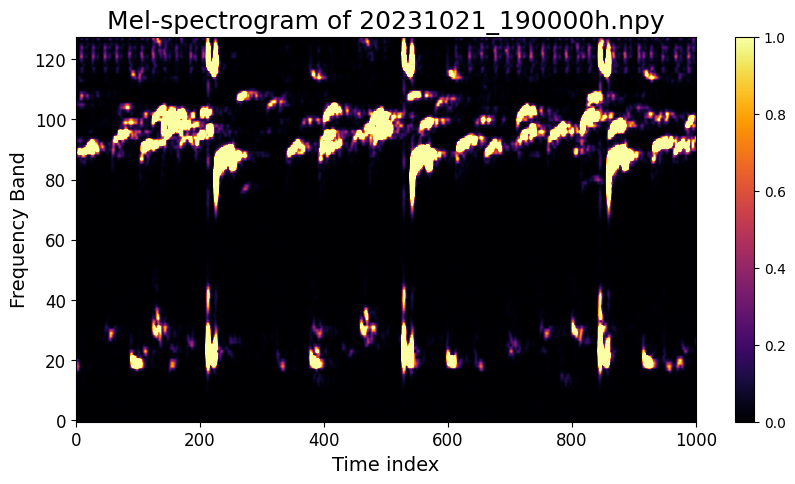
\includegraphics[width=0.9\linewidth]{Graphics/mel-spectrogram.png}
  \caption{Mel-espectrograma de un fragmento del audio \texttt{20231021\_190000h}, donde se observan las notas “CO” (baja frecuencia) y “LIN” (alta frecuencia).}
  \label{fig:mel_example}
\end{figure}






% region noise
\section{Filtrado de ruido de fondo}
\label{sec:filtrado}


Para garantizar que las características acústicas extraídas 
representaran de manera fidedigna la emisión vocal de los 
Colines, se implementó una etapa de eliminación de 
ruido dirigida a atenuar tanto interferencias puntuales (por 
ejemplo, vocalizaciones de otras especies o clics mecánicos) 
como ruidos persistentes de banda ancha (motores de vehículos, 
canto de grillos, viento). En la 
Figura \ref{fig:car} se muestra el Mel-espectrograma de un 
fragmento del audio \texttt{20231021\_190000b}, en el que se registró el ruido generado por el paso 
de un automóvil cercano.


\begin{figure}[ht]
    \centering
    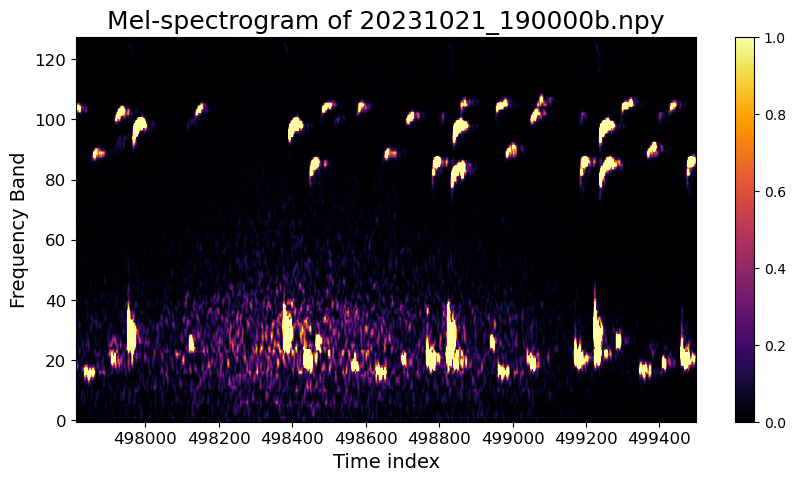
\includegraphics[width=\columnwidth]{Graphics/car_noise_before.png}
    \caption{Mel-espectrograma del fragmento del audio \texttt{20231021\_190000b}, en el que aparece el ruido de un motor de automóvil. Antes del filtrado.}
    \label{fig:car}
\end{figure}

La técnica empleada consistió en una poda espectral (o \emph{spectral pruning}) basada en 
el percentil 99.9 de la amplitud por frecuencia. 
Para cada grabación se calculó el 
espectrograma de potencia y, en cada banda de frecuencia, se 
determinó el valor correspondiente al percentil 99.9 de la 
amplitud a lo largo de todo el período analizado. 
A continuación, se descartaron todas las componentes espectrales 
por 
debajo de ese umbral, reteniendo solo los eventos acústicos 
cuyas intensidades superaron el fondo de ruido común.
En la Figura \ref{fig:car2} se presenta el Mel-espectrograma
del mismo fragmento de audio que se muestra en la Figura \ref{fig:car},
pero luego de aplicar el filtrado.

\begin{figure}[ht]
    \centering
    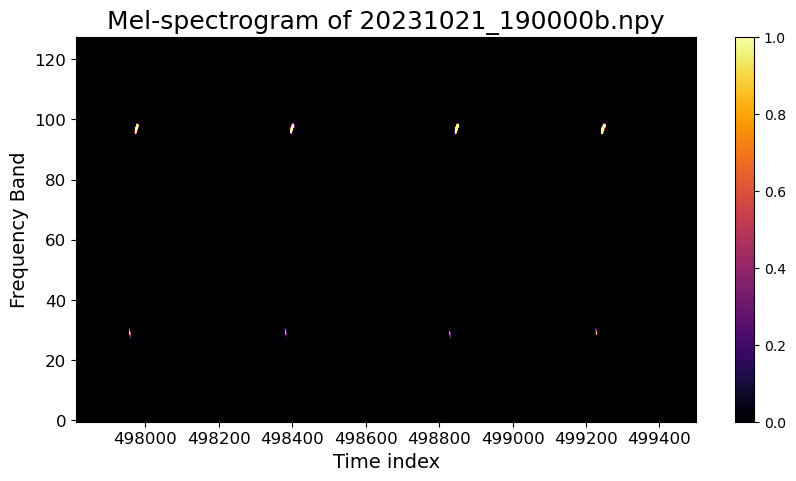
\includegraphics[width=\columnwidth]{Graphics/car_noise_after.png}
    \caption{Mel-espectrograma del fragmento del audio \texttt{20231021\_190000b}, en el que se registró el ruido de un motor de automóvil. Después del filtrado.}
    \label{fig:car2}
\end{figure}

Este procedimiento permitió suprimir eficazmente las 
componentes de baja energía asociadas al ruido ambiental no 
informativo y conservar las estructuras espectrales dominantes 
de los cantos de \emph{E.\,eileenae}.




% region sync
% \section{Sincronización de los audios}
% \label{sec:sincronizacion}


% La sincronización de las grabaciones de audio constituyó una 
% etapa crítica para asegurar la coherencia temporal necesaria en 
% el análisis posterior de los cantos de \emph{E.\,eileenae}. 
% Aunque los nueve dispositivos de grabación fueron activados 
% simultáneamente, cada uno presentaba desfases mínimos, posiblemente 
% debido a pequeñas variaciones en el hardware y el error de 
% la activación remota, los cuales 
% resultaban significativos para el procesamiento posterior. 
% Para corregir estos 
% desfases, se implementó un procedimiento automático basado en 
% señales de energía derivadas de los Mel-espectrogramas de cada 
% canal.

% En primer lugar, se calculó la energía temporal de cada 
% Mel-espectrograma, obteniendo en cada instante \(j\), la suma 
% de los cuadrados de las intensidades en las \(n\) bandas de 
% frecuencia:
% \begin{equation}
%     \label{energyformula}
%     E_j \;=\; \sum_{i=0}^{n} a_{ij}^2 
%     \qquad\forall\,j,
% \end{equation}
% donde \(a_{ij}\) es la intensidad en la banda \(i\) y el tiempo 
% \(j\), y \(E_j\) representa la energía total en dicho instante 
% \cite{jurafskyspeech}. 
% En la Figura \ref{fig:energy} se aprecia la evolución de 
% \(E_j\) para el canal “\texttt{20231021\_190000h}”.



% \begin{figure}[ht]
%     \centering
%     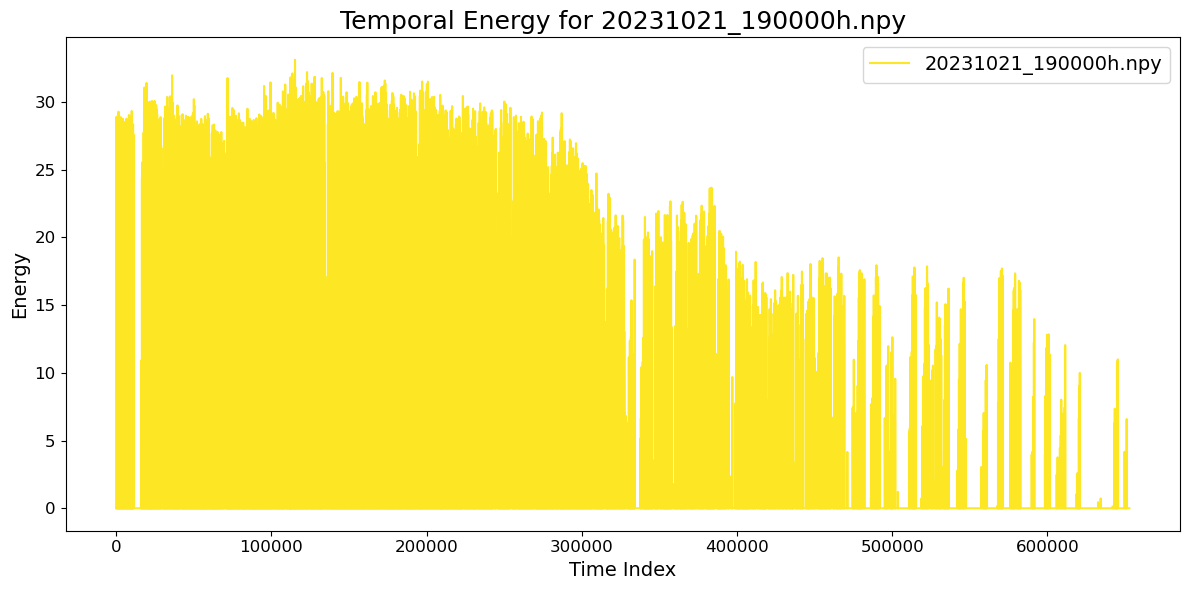
\includegraphics[width=0.9\linewidth]{Graphics/temp_energy.png}
%     \caption{Energía temporal del audio \texttt{20231021\_190000h}.}
%     \label{fig:energy}
%   \end{figure}

% A continuación, se detectaron los picos locales de \(E_j\) 
% mediante una función que localiza 
% máximos relativos en una secuencia discreta, ajustando 
% parámetros de prominencia y distancia mínima para evitar falsas 
% detecciones debidas a ruido residual \cite{scipy-signal}. 
% En la Figura\ref{fig:peaks} se muestran los momentos de pico de 
% energía de un fragmento del audio \texttt{20231021\_190000h}.

% \begin{figure}[ht]
%     \centering
%     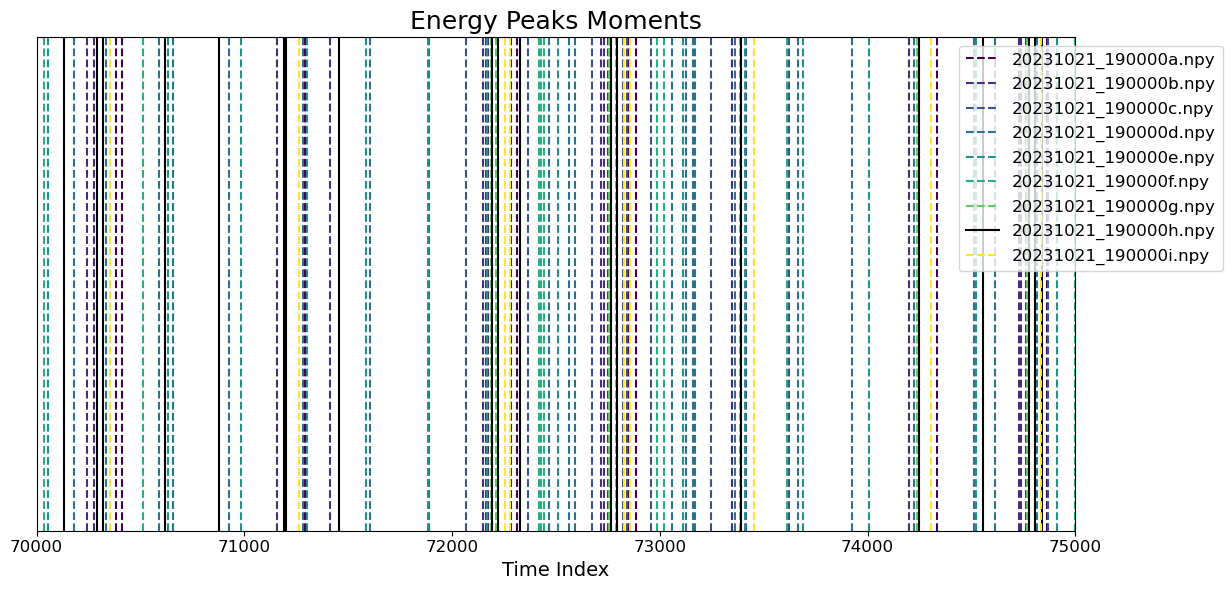
\includegraphics[width=0.9\linewidth]{Graphics/peaks_before.png}
%     \caption{Momentos de pico de energía de un fragmento de los audios del \texttt{20231021\_190000} antes de sincronizar. Con línea discontinua se representa el momento de tiempo en que ocurre un pico de energía para cada audio, que se puede distinguir de los demás por el color de la línea. Con línea continua negra se representan en particular los momentos de pico de energía de la grabación \texttt{20231021\_190000h}.}
%     \label{fig:peaks}
%   \end{figure}

% Para estimar los desfases entre canales, se construyó un 
% histograma de los tiempos de pico de cada audio, relativo al 
% inicio de la grabación. Luego, se aplicó correlación cruzada \cite{costa2021comparing} 
% entre los histogramas de pares de canales, desplazando uno 
% respecto al otro y calculando el coeficiente de correlación 
% máxima para cada posible \emph{lag}. 
% Este enfoque permitió identificar el desfase 
% óptimo que maximiza el solapamiento de las estructuras 
% temporales de canto.

% Una vez determinados los desfases relativos, se alinearon todos 
% los canales utilizando un canal de referencia global (en este caso, el canal 
% “\texttt{20231021\_190000h}”, que presentaba la señal más limpia) aplicando un 
% desplazamiento de muestras correspondiente al \emph{lag} 
% calculado. La Figura \ref{fig:peaksafter} ilustra los picos de 
% energía tras la alineación, mostrando una coincidencia temporal 
% precisa. Finalmente, estos desfases se incorporaron a 
% los archivos originales, de modo que todos los 
% audios quedaran sincronizados con un error mínimo.


% \begin{figure}[ht]
%     \centering
%     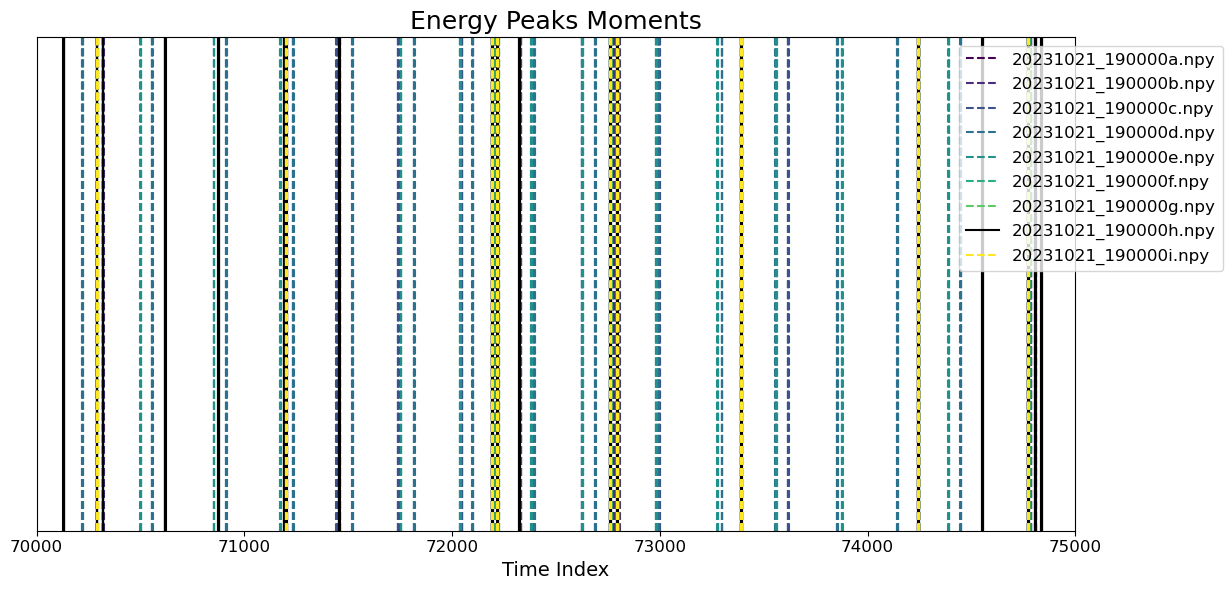
\includegraphics[width=0.9\linewidth]{Graphics/peaks_after.png}
%     \caption{Momentos de pico de energía de un fragmento de los audios del \texttt{20231021\_190000} después de sincronizar. Con línea discontinua se representa el momento de tiempo en que ocurre un pico de energía para cada audio, que se puede distinguir de los demás por el color de la línea. Con línea continua negra se representan en particular los momentos de pico de energía de la grabación \texttt{20231021\_190000h}}
%     \label{fig:peaksafter}
%   \end{figure}

\section{Sincronización de los audios}
\label{sec:sincronizacion}

La sincronización de las grabaciones de audio constituyó una 
etapa crítica para asegurar la coherencia temporal necesaria en 
el análisis posterior de los cantos de \emph{E.\,eileenae}. 
Aunque los nueve dispositivos de grabación fueron activados 
simultáneamente, cada uno presentaba desfases mínimos, posiblemente 
debido a pequeñas variaciones en el hardware y al retardo de 
la activación remota, los cuales 
resultaban significativos para el procesamiento subsecuente. 
Para corregir estos 
desfases se implementó un procedimiento automático basado en 
los puntos de máximos locales extraídos de los Mel-espectrogramas de cada 
canal.

En primer lugar, tras eliminar el ruido de fondo, se localizaron 
los puntos de máximo local en cada espectrograma. Dado que un 
Mel-espectrograma es una matriz de dimensiones (bandas de frecuencias x tiempo), 
cada punto de máximo se identifica por un par \((t,f)\), donde 
\(t\) es el índice temporal y \(f\) la banda de frecuencia 
asociada.

A continuación, para cada par de archivos se tomaron sus 
respectivas listas de puntos de máximo local y se alinearon en 
tiempo buscando el desplazamiento óptimo. Con tal fin, se 
construyeron histogramas de los índices temporales de los 
máximos (ignorando la componente de frecuencia) y se aplicó 
correlación cruzada entre ambos histogramas. 
La correlación cruzada es una medida estadística que cuantifica 
la similitud entre dos señales al compararlas en diferentes 
desplazamientos temporales, utilizada comúnmente para sincronizar 
grabaciones o identificar patrones coincidentes en análisis de 
series temporales. Se calcula con la siguiente fórmula:
\begin{equation*}
	CC = \sum_{i=0}^{n} a_{i}b_{i},     \cite{costa2021comparing}
\end{equation*} 
donde $a_i$ y $b_i$ son los valores en el índice $i$ de los \textit{arrays} sobre los que se aplica el método.
En este caso el desplazamiento (\emph{lag}) que maximiza la correlación 
indica la mejor coincidencia temporal entre los picos de energía 
de los dos canales.

Una vez obtenidos los \emph{lags} óptimos para cada par de 
archivos, se empleó un algoritmo \textit{greedy} para propagar 
estas alineaciones y establecer una sincronización global entre 
los nueve canales. Finalmente, los desplazamientos resultantes 
se aplicaron a los datos originales, garantizando que todos los 
audios compartieran una referencia temporal común con un error 
mínimo.

% En la Figura~\ref{fig:peaksbefore} se muestran los picos de 
% energía antes de sincronizar, mientras que la 
% Figura~\ref{fig:peaksafter} ilustra la coincidencia de los 
% máximos tras aplicar los \emph{lags} y completar el alineamiento 
% global.

% \begin{figure}[ht]
%     \centering
%     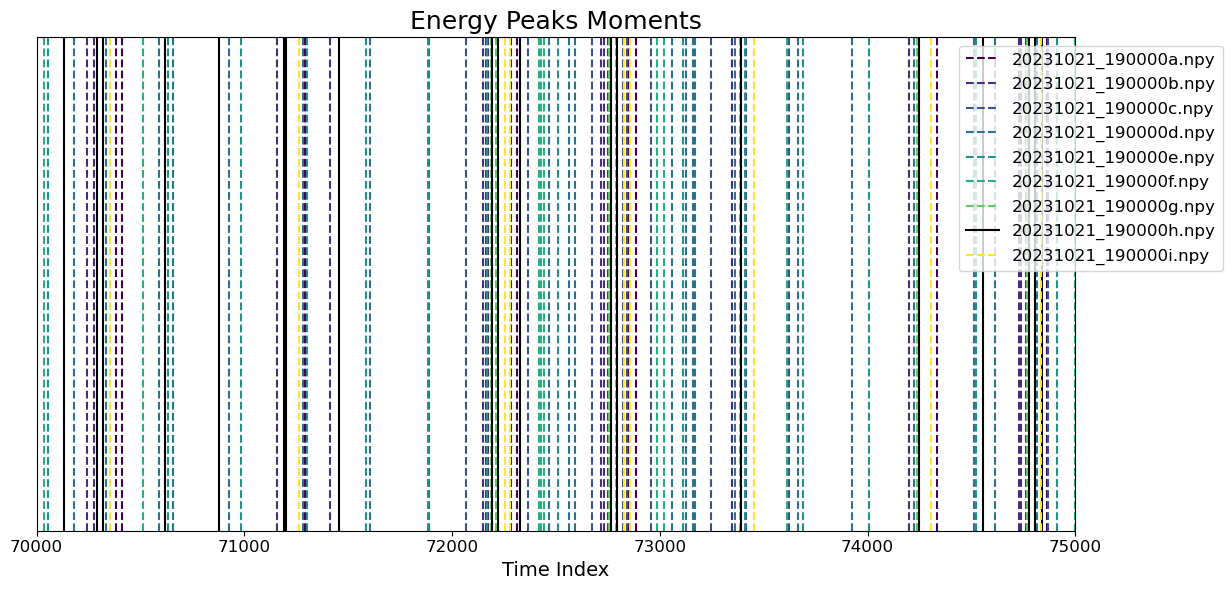
\includegraphics[width=0.9\linewidth]{Graphics/peaks_before.png}
%     \caption{Momentos de pico de energía de un fragmento de los audios del \texttt{20231021\_190000} antes de sincronizar. La línea continua negra muestra los picos del canal de referencia (\texttt{...h}), y las discontinuas los de los demás canales.}
%     \label{fig:peaksbefore}
% \end{figure}

% \begin{figure}[ht]
%     \centering
%     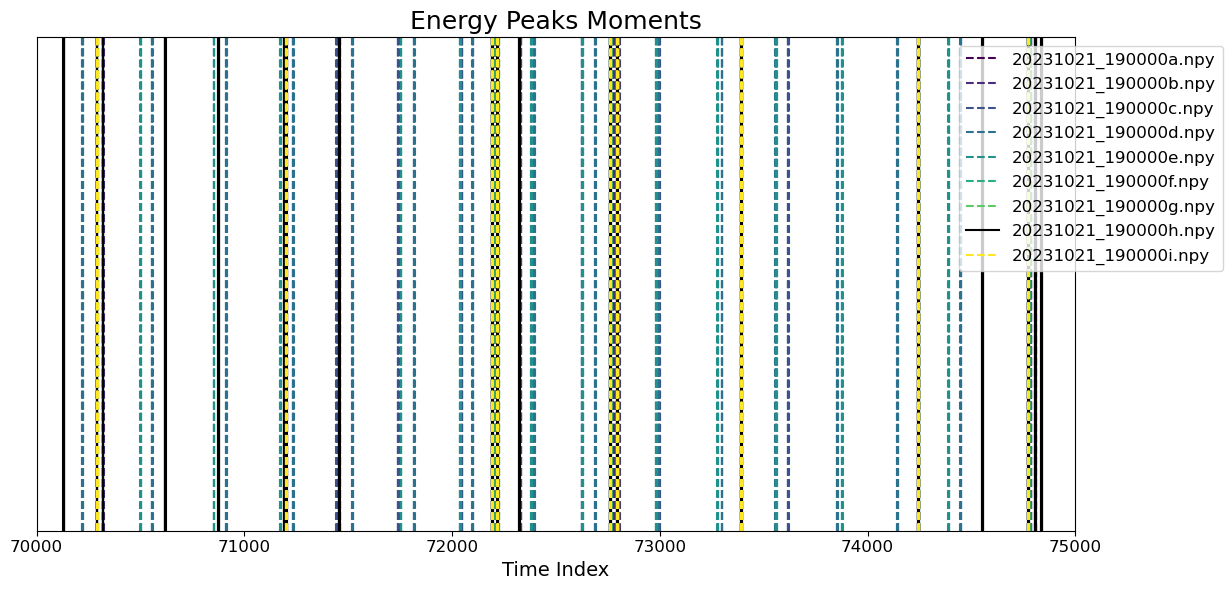
\includegraphics[width=0.9\linewidth]{Graphics/peaks_after.png}
%     \caption{Momentos de pico de energía del mismo fragmento después de aplicar la alineación global de \emph{lags}. Todas las trazas coinciden temporalmente.}
%     \label{fig:peaksafter}
% \end{figure}



% region algorythms
\section{Detección y asignación heurística de cantos de Colines a Micrófonos}
\label{sec:deteccion_asignacion}


Para obtener un \emph{dataset} con el que fuera posible llevar a cabo 
los estudios de comportamiento de los coros, 
se hizo imprescindible diseñar procesos automáticos 
capaces de extraer, a partir de las grabaciones sincronizadas y 
filtradas, las series temporales de emisión de cada Colín,
asignando correctamente cada canto a su respectivo micrófono.
Solo disponiendo de estas secuencias individuales se puede 
avanzar hacia un análisis riguroso de las interacciones 
acústicas y las dinámicas de grupo, ya que cualquier estudio
de causalidad o modelado de red requiere un 
sistema de eventos bien definido y libre de ambigüedades en la 
identificación de los emisores. En esta sección se presentan 
dos algoritmos heurísticos que, partiendo de Mel-espectrogramas, 
automatizaron la detección de instantes de 
canto y su asignación espacial, constituyendo la base 
metodológica para el posterior estudio de las redes de 
interacción en el coro de \emph{E.\,eileenae}.



\subsection{Algoritmo basado en hipótesis de energías relativas}
\label{sec:alg_energia}

El método propuesto se sustenta en la suposición de que
para un micrófono, los cantos del individuo más cercano deben ser registrados con las
mayores energías relativas a dicho micrófono. Por lo tanto, si en cada uno se identifican 
los momentos de mayor energía y se elimina la información de esos cantos de las demás grabaciones,
se obtendrán por separado los datos que se buscan.
Para explotar esta idea se dividió cada 
grabación en dos bandas de interés (baja frecuencia (“CO”) y 
alta frecuencia (“LIN”)) y se procesaron en paralelo. En cada 
banda se computaron las energías temporales, 
obteniendo en cada instante \(j\), la suma 
de los cuadrados de las intensidades en las \(n\) bandas de 
frecuencia del Mel-espectrograma, es decir:
\begin{equation}
    \label{energyformula}
    E_j \;=\; \sum_{i=0}^{n} a_{ij}^2 
    \qquad\forall\,j,
\end{equation}
donde \(a_{ij}\) es la intensidad en la banda \(i\) y el tiempo 
\(j\), y \(E_j\) representa la energía total en dicho instante 
\cite{jurafskyspeech}. 


A partir de estos vectores de energía, el algoritmo aplicó la 
siguiente estrategia:

\begin{enumerate}
  \item Se creó un \emph{array} de ceros para cada micrófono, que almacenaría la energía del canto asignado en cada instante.
  \item Mientras existieran valores no nulos en los vectores de energía originales:
  \begin{itemize}
    \item Se seleccionó aleatoriamente uno de los nueve canales. (Esta selección aleatoria permite que si dos cantos pertenecientes a individuos distintos se multiplexan en tiempo, se guarde la información de ambos en el \emph{dataset} final.)
    \item Se halló la posición \(j^*\) de la energía máxima en ese canal.
    \item Se guardó el valor de dicha energía en la posición \(j^*\) del \emph{array} de resultados para ese micrófono.
    \item Se estableció a cero el valor de la energía en la posición \(j^*\) de todos los vectores, eliminando así la contribución de ese canto para las demás grabaciones.
  \end{itemize}
  \item El proceso se repitió hasta que todos los vectores de energía quedaron vacíos.
  \item Finalmente, se almacenaron los \emph{arrays} resultantes como secuencias de cantos por micrófono.
\end{enumerate}


\begin{algorithm}
    \caption{Colin Sequence by Energy}
    \begin{algorithmic}[1]
    \Require 
      Temporal energies \(\{E^{(k)}\}_{k=1}^9\), length \(N\)
    \Ensure
      Calls sequences \(\{S^{(k)}\}_{k=1}^9\)
    \State Initialize \(S^{(k)} \leftarrow [0,\dots,0]\) for \(k=1,\dots,9\)
    \While{\(\exists\,k,j \;|\; E^{(k)}_j>0\)}
      \State Select randomly \(k\in\{1,\dots,9\}\)
      \State \(j^* \leftarrow \arg\max_j E^{(k)}_j\)
      \State \(S^{(k)}_{j^*} \leftarrow E^{(k)}_{j^*}\)
      \Comment{Save maximum value to file}
      \For{each \(k'=1,\dots,9\)}
      \Comment{Erase value from all arrays}
        \State \(E^{(k')}_{j^*} \leftarrow 0\)
      \EndFor
    \EndWhile
    \State \Return \(\{S^{(k)}\}\)
    \end{algorithmic}
\end{algorithm}

Este procedimiento, ilustrado en el pseudocódigo del 
Algoritmo 1, garantizó que cada instante de canto fuera 
asignado al micrófono cuya energía fuera dominante. 
La complejidad temporal resultó \(O(n^2)\), con \(n\) igual al 
número de muestras en el eje temporal del Mel-espectrograma.



\subsection{Algoritmo basado en agrupamiento espectro-temporal}
\label{sec:alg_aglomerativo}

El segundo método propuesto partió también de los 
Mel-espectrogramas preprocesados y filtrados, pero incorporó 
explícitamente la estructura temporal y espectral de los cantos 
“CO” y “LIN” de \emph{E.\,eileenae}. La idea central consistió 
en extraer todos los máximos locales del espectrograma (cada 
uno identificado por un par \((t,f)\)) y luego agruparlos en 
parejas correspondientes a los dos componentes del canto 
(frecuencia baja para “CO” y alta para “LIN”) de acuerdo con 
ventanas temporales aprendidas a partir de histogramas de datos 
manuales. A las parejas \((t_{\mathrm{CO}},f_{\mathrm{CO}})\) y 
\((t_{\mathrm{LIN}},f_{\mathrm{LIN}})\) obtenidas se les aplicó 
un algoritmo aglomerativo de clustering, usando como métrica la 
suma de cuadrados de la diferencia de frecuencias, de modo que 
aquellas parejas cuyos valores espectrales y temporales se 
encontraran más cercanos quedaran agrupadas. Cada grupo 
resultante definió una hipótesis de secuencia de canto, a la que 
se asignó la potencia media más alta como criterio de selección 
de la rana más cercana. Finalmente, los canales en los que el 
número de máximos agrupados no alcanzó un umbral mínimo fueron 
descartados, asumiendo la ausencia de un Colín próximo.
A continuación se describen los pasos seguidos, también 
ilustrados en el pseudocódigo del Algoritmo 2.

\begin{enumerate}
  \item Se calculó el Mel-espectrograma de cada archivo.
  \item Se localizaron todos los máximos locales del Mel-espectrograma, cada uno especificado por un par \((t,f)\).
  \item Se filtraron aquellos máximos cuyas frecuencias y tiempos coincidían con los rangos propios de las notas “CO” y “LIN”, según los histogramas derivados de datos reales.
  \item A las parejas \((t_{\mathrm{CO}},f_{\mathrm{CO}})\) y \((t_{\mathrm{LIN}},f_{\mathrm{LIN}})\) resultantes se les aplicó clustering aglomerativo, con distancia basada en la diferencia al cuadrado de frecuencias.
  \item Se seleccionó la secuencia cuyo grupo presentó la potencia media de canto más alta, asignándola al micrófono correspondiente.
  \item Se descartaron los canales con un número de máximos inferior al umbral mínimo, declarándolos sin detección de Colín.
\end{enumerate}


\begin{algorithm}[H]
\caption{Spectral-Time Clustering Algorithm for Frog Call Detection}
\begin{algorithmic}[1]
\Require Audio files \texttt{audio\_files}, minimum cluster size threshold \texttt{min\_threshold}
\For{\texttt{each audio\_file in audio\_files}}
    \State Compute Mel-spectrogram: \texttt{S = melspectrogram(audio\_file)}
    \State Identify all local maxima in \texttt{S} as pairs $(t, f)$
    \State Filter maxima to keep only those within CO and LIN frequency and time ranges based on annotated histograms
    \State Group pairs $(t_{\text{CO}}, f_{\text{CO}})$ and $(t_{\text{LIN}}, f_{\text{LIN}})$ into sequences
    \State Apply agglomerative clustering to these sequences using squared frequency difference as distance metric
    \State Compute mean power for each cluster
    \If{maximum cluster size $<$ \texttt{min\_threshold}}
        \State Discard this audio file (no frog detected)
    \Else
        \State Assign the cluster with the highest mean power to this microphone
    \EndIf
\EndFor
\end{algorithmic}
\end{algorithm}



% region Ising
\section{Modelado de interacciones con el modelo de Ising}
\label{sec:modelado_ising}



El análisis de las dinámicas colectivas de los Colines requiere un 
marco formal capaz de capturar las dependencias entre los 
individuos a partir de observaciones de su comportamiento 
acústico. En esta sección se describe el uso del modelo de 
Ising como herramienta para representar y cuantificar las 
interacciones entre machos vocalizantes, siguiendo un enfoque 
basado en inferencia estadística y física computacional.

\subsection{Fundamentos del modelo de Ising}

El modelo de Ising fue concebido por Wilhelm Lenz e introducido por Ernst Ising en 1925 como 
una simplificación del comportamiento colectivo de espines en 
materiales ferromagnéticos \cite{ising1925beitrag}. En su 
formulación clásica, cada componente del sistema está 
representado por una variable binaria \( \sigma_i \in \{-1, +1\} \), 
que puede interpretarse como un estado de activación 
(por ejemplo, presencia o ausencia de vocalización). Las 
interacciones entre pares de componentes se codifican mediante 
parámetros \( J_{ij} \), que determinan si las unidades tienden 
a sincronizarse o a inhibirse mutuamente, mientras que un 
parámetro \( h_i \) refleja la predisposición individual (o 
sesgo) del componente \( i \) a estar activo.

El conjunto de estados del sistema está dado por el vector 
binario 
\(\boldsymbol{\sigma} = (\sigma_1, \dots, \sigma_N)\), y la 
probabilidad de observar una configuración determinada se modela 
según la distribución de Boltzmann:
\[
P(\boldsymbol{\sigma}) = \frac{1}{Z} \exp\left( \sum_{i<j} J_{ij} \sigma_i \sigma_j + \sum_{i} h_i \sigma_i \right),
\]
donde \( Z \) es la función de partición que normaliza la 
distribución:
\[
Z = \sum_{\boldsymbol{\sigma}} \exp\left( \sum_{i<j} J_{ij} \sigma_i \sigma_j + \sum_i h_i \sigma_i \right).
\]

Esta formulación permite representar redes de interacciones con 
estructuras arbitrarias, haciendo del modelo de Ising una 
herramienta versátil que ha sido empleada exitosamente en áreas 
como neurociencia, genética, economía y análisis de redes 
sociales \cite{chau2017inverse}.

\subsection{Formulación del sistema acústico como red de espines}

Para modelar los coros de \emph{E.\,eileenae}, se asumió que 
cada uno de los nueve individuos registrados corresponde a un 
nodo del sistema, y su comportamiento acústico en un instante 
dado queda representado por un espín \( \sigma_i \in \{-1, +1\} \), 
donde \( +1 \) indica que el individuo está emitiendo un canto 
y \( -1 \) que permanece en silencio.

Las configuraciones \(\boldsymbol{\sigma}\) fueron extraídas a 
partir de las secuencias temporales de detección previamente 
construidas, 
dividiendo el tiempo en intervalos discretos (frames) de 
longitud fija. Cada configuración refleja el estado coral del 
sistema en un instante, y el conjunto de configuraciones 
observado se utilizó como base para inferir los parámetros 
\( \{J_{ij}\} \) y \( \{h_i\} \) que describen la estructura de 
interacción y la propensión individual a cantar.

Aunque el sistema de cantos no necesariamente satisface los 
criterios de equilibrio termodinámico, se adoptó esta suposición 
como primera aproximación, lo cual permitió el uso de 
herramientas formales del marco de física estadística 
\cite{zeng2013maximum}. Esta simplificación habilita una 
descripción cuantitativa de las correlaciones observadas, útil 
para identificar influencias directas entre individuos del coro.

\subsection{Inferencia por máxima verosimilitud y descenso por 
gradiente}

La tarea de inferir los parámetros del modelo a partir de 
observaciones consiste en encontrar los valores de \( J_{ij} \) 
y \( h_i \) que maximizan la verosimilitud del conjunto de 
configuraciones observadas:
\[
\mathcal{L}(J, h) = \sum_{m=1}^{M} \log P(\boldsymbol{\sigma}^{(m)}),
\]
donde \( \{\boldsymbol{\sigma}^{(m)}\}_{m=1}^M \) son las 
configuraciones registradas.

El gradiente de esta función de verosimilitud con respecto a los 
parámetros tiene la forma:
\[
\frac{\partial \mathcal{L}}{\partial J_{ij}} = \langle \sigma_i \sigma_j \rangle_{\text{datos}} - \langle \sigma_i \sigma_j \rangle_{\text{modelo}},
\]
\[
\frac{\partial \mathcal{L}}{\partial h_i} = \langle \sigma_i \rangle_{\text{datos}} - \langle \sigma_i \rangle_{\text{modelo}},
\]
donde los términos \( \langle \cdot \rangle_{\text{datos}} \) se 
obtienen como promedios sobre las configuraciones empíricas, y 
los términos \( \langle \cdot \rangle_{\text{modelo}} \) se 
calculan a partir de la distribución del modelo.

En este trabajo, gracias al tamaño reducido del sistema (9 
nodos, \(2^9 = 512\) configuraciones), fue posible calcular de 
forma exacta la función de partición y las expectativas 
modeladas, evitando el uso de muestreo estocástico como Monte 
Carlo \cite{pena2001deduccion}. Esto permitió implementar un algoritmo de descenso por 
gradiente exacto, complementado con regularización \(L_2\) sobre 
los pesos \( J_{ij} \) para evitar sobreajuste.

La energía asociada a una configuración se definió como:
\[
E(\boldsymbol{\sigma}) = -\sum_{i<j} J_{ij} \sigma_i \sigma_j - \sum_i h_i \sigma_i,
\]
lo cual permitió expresar su probabilidad como:
\[
P(\boldsymbol{\sigma}) = \frac{1}{Z} \exp\left(-E(\boldsymbol{\sigma})\right).
\]

El algoritmo iterativo actualizó los parámetros siguiendo las 
reglas:
\begin{align}
    h_i &\leftarrow h_i + \eta \left( \langle \sigma_i \rangle_{\text{datos}} - \langle \sigma_i \rangle_{\text{modelo}} \right), \\
    J_{ij} &\leftarrow J_{ij} + \eta \left( \langle \sigma_i \sigma_j \rangle_{\text{datos}} - \langle \sigma_i \sigma_j \rangle_{\text{modelo}} \right) - \eta \lambda J_{ij},
\end{align}
donde \( \eta \) es la tasa de aprendizaje y \( \lambda \) el 
coeficiente de regularización. Además para el cálculo de las correlaciones
empíricas se utilizó un \(\Delta t = 0\), es decir, se tuvo en cuenta que cada
estado era el valor de canto o no canto (+1 o -1) en un instante de tiempo.

\begin{algorithm}[H]
    \caption{Gradient Descent for Ising Model Parameter Inference}
    \begin{algorithmic}[1]
    \Require Observed configurations \( \{\boldsymbol{\sigma}^{(1)}, \dots, \boldsymbol{\sigma}^{(M)}\} \), learning rate \( \eta \), number of iterations \( T \), regularization parameter \( \lambda \)
    \State Initialize \( h_i \gets 0 \), \( J_{ij} \gets 0 \) for all \( i, j \)
    \For{$t \gets 1$ to $T$}
        \State Compute empirical averages:
            \[ \langle \sigma_i \rangle_{\text{data}}, \quad \langle \sigma_i \sigma_j \rangle_{\text{data}} \]
        \State Enumerate all configurations \( \boldsymbol{\sigma} \in \{-1, +1\}^9 \)
        \For{each configuration \( \boldsymbol{\sigma} \)}
            \State Compute energy: 
                \[ E(\boldsymbol{\sigma}) = -\sum_{i<j} J_{ij} \sigma_i \sigma_j - \sum_i h_i \sigma_i \]
            \State Compute unnormalized probability: 
                \[ \tilde{P}(\boldsymbol{\sigma}) = \exp(-E(\boldsymbol{\sigma})) \]
        \EndFor
        \State Normalize to obtain \( P(\boldsymbol{\sigma}) \)
        \State Compute model expectations:
            \[ \langle \sigma_i \rangle_{\text{model}}, \quad \langle \sigma_i \sigma_j \rangle_{\text{model}} \]
        \State Update parameters:
            \[
            h_i \gets h_i + \eta \left( \langle \sigma_i \rangle_{\text{data}} - \langle \sigma_i \rangle_{\text{model}} \right)
            \]
            \[
            J_{ij} \gets J_{ij} + \eta \left( \langle \sigma_i \sigma_j \rangle_{\text{data}} - \langle \sigma_i \sigma_j \rangle_{\text{model}} \right) - \eta \lambda J_{ij}
            \]
    \EndFor
    \end{algorithmic}
\end{algorithm}

Este procedimiento (descrito en el pseudocódigo del Algoritmo 3) garantizó la convergencia a un conjunto de 
parámetros que maximizan la verosimilitud del modelo, y 
proporciona una primera reconstrucción de la red de 
interacciones acústicas dentro del coro.
